% Capitolo da inserire in un documento che carichi almeno:
% \usepackage{amsmath}
% \usepackage{xcolor}
% \usepackage{listings}
% \usepackage{booktabs}
%
% Si assume inoltre che sia definito uno stile listings per Python.

\chapter{Istogrammi e fit gaussiani con Python}
\label{chap:istogrammi-fit}

\section{Introduzione}

Un istogramma rappresenta la distribuzione di un insieme di dati numerici.
L'intervallo compreso tra il valore minimo e il valore massimo viene
suddiviso in sottointervalli, detti \emph{bin}. Per ogni bin si conta il
numero di dati che ricadono al suo interno.

Se indichiamo con $N_i$ il numero di elementi contenuti nel bin $i$,
l'istogramma è costituito dalla sequenza dei conteggi

\[
N_1,N_2,\ldots,N_m,
\]

dove $m$ è il numero complessivo dei bin.

L'altezza di ciascuna barra rappresenta quindi una frequenza assoluta.
L'asse orizzontale riporta i valori della variabile osservata, mentre
l'asse verticale riporta il numero di osservazioni contenute in ciascun
intervallo.

In questo capitolo si costruirà un istogramma per gradi:

\begin{enumerate}
    \item calcolo manuale dei conteggi;
    \item uso elementare di \texttt{plt.hist};
    \item aggiunta delle etichette degli assi;
    \item scelta del numero di bin e personalizzazione grafica;
    \item recupero dei conteggi e dei bordi dei bin;
    \item sovrapposizione di un fit gaussiano.
\end{enumerate}

\section{Costruzione manuale: \texttt{istogrammamimano.py}}

Il primo script costruisce i conteggi senza utilizzare NumPy o
Matplotlib per il calcolo dell'istogramma.

\begin{lstlisting}[language=Python]
def istogrammello(data, div):
    high = max(data) + 0.01
    low = min(data) - 0.01
    delta = (high - low) / div

    hist = []

    for a in range(div):
        hist.append(0.)

    for a in data:
        for b in range(div):
            if a > low + b*delta and a <= low + (b+1)*delta:
                hist[b] = hist[b] + 1

    return hist


dati = list(
    map(
        float,
        open("daterelli.dat").read().strip().split()
    )
)

histo = istogrammello(dati, 10)

for a in histo:
    print(a)
\end{lstlisting}

\subsection{Argomenti della funzione}

La funzione

\begin{lstlisting}[language=Python]
def istogrammello(data, div):
\end{lstlisting}

riceve due argomenti:

\begin{itemize}
    \item \texttt{data}: la sequenza dei dati numerici;
    \item \texttt{div}: il numero di intervalli nei quali dividere il
          campo dei dati.
\end{itemize}

\subsection{Estremi dell'intervallo}

Le istruzioni

\begin{lstlisting}[language=Python]
high = max(data) + 0.01
low = min(data) - 0.01
\end{lstlisting}

calcolano gli estremi superiore e inferiore. Il piccolo margine aggiunto
agli estremi riduce il rischio che il valore minimo o massimo rimanga
escluso a causa delle disuguaglianze usate nella selezione.

La larghezza comune dei bin è

\[
\Delta = \frac{x_{\max}-x_{\min}}{m},
\]

ed è calcolata da

\begin{lstlisting}[language=Python]
delta = (high - low) / div
\end{lstlisting}

Tutti i bin hanno quindi la stessa larghezza.

\subsection{Inizializzazione dei conteggi}

La lista dei conteggi è inizialmente vuota:

\begin{lstlisting}[language=Python]
hist = []
\end{lstlisting}

Il primo ciclo inserisce un valore nullo per ogni bin:

\begin{lstlisting}[language=Python]
for a in range(div):
    hist.append(0.)
\end{lstlisting}

Se \texttt{div=10}, al termine del ciclo la lista contiene dieci zeri.
Il valore \texttt{hist[b]} memorizzerà il numero di dati appartenenti al
bin $b$.

\subsection{Assegnazione dei dati ai bin}

Il doppio ciclo

\begin{lstlisting}[language=Python]
for a in data:
    for b in range(div):
\end{lstlisting}

considera ogni dato \texttt{a} e controlla tutti i bin. Il dato appartiene
al bin $b$ se soddisfa

\[
x_{\min}+b\Delta < a
\leq x_{\min}+(b+1)\Delta.
\]

Nel codice:

\begin{lstlisting}[language=Python]
if a > low + b*delta and a <= low + (b+1)*delta:
    hist[b] = hist[b] + 1
\end{lstlisting}

Quando la condizione è vera, il conteggio del bin viene incrementato di
uno.

\begin{figure}[htbp]
\centering
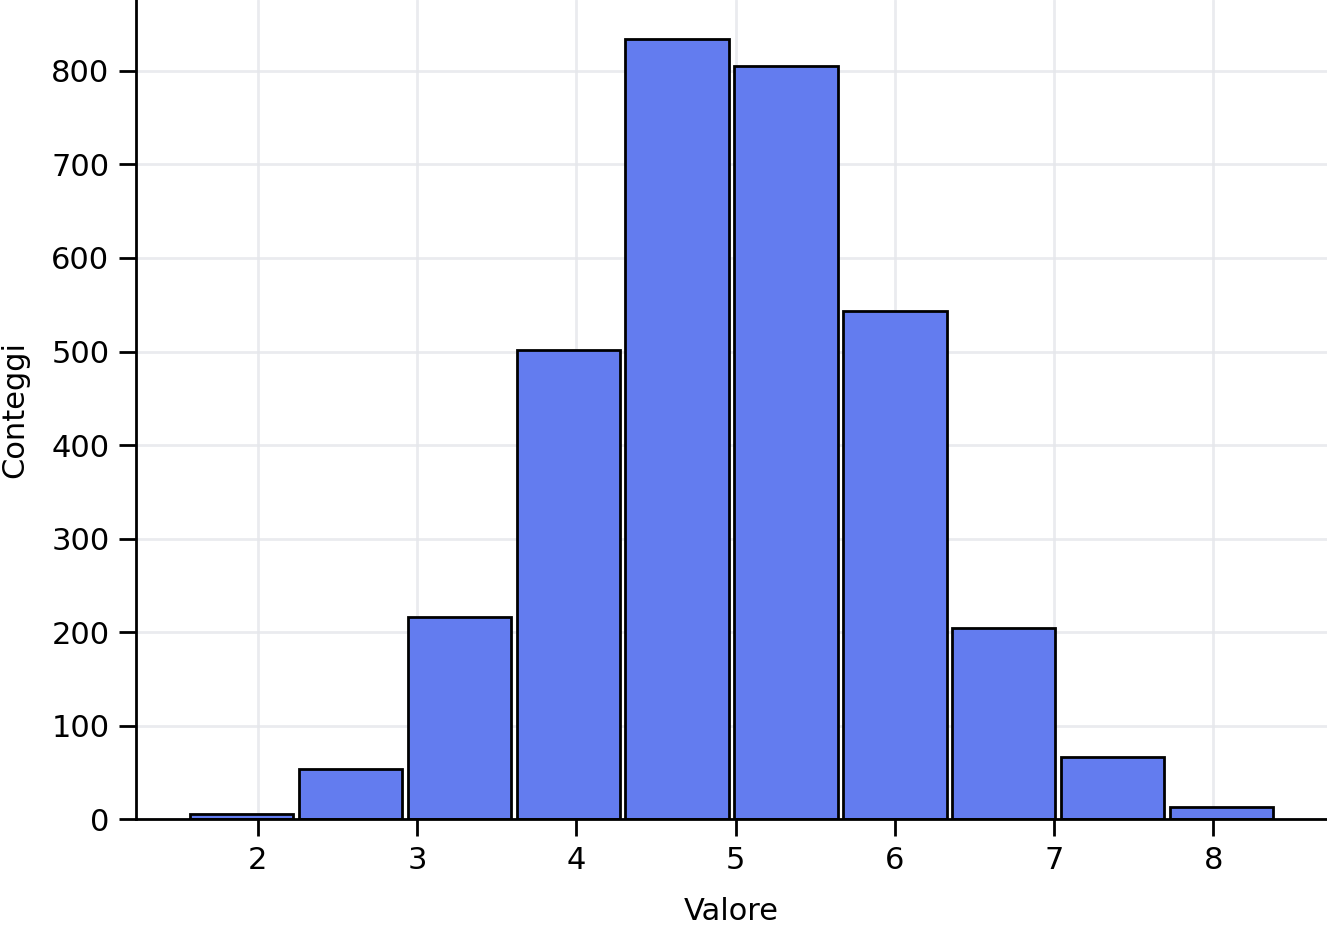
\includegraphics[width=0.78\textwidth]{fig_istogramma_manuale.png}
\caption{Rappresentazione grafica dei conteggi calcolati manualmente da \texttt{istogrammamimano.py}.}
\label{fig:istogramma-manuale}
\end{figure}

Questo algoritmo è didatticamente utile perché mostra come nasce un
istogramma. Non è però efficiente: per $N$ dati e $m$ bin esegue fino a
$N\times m$ confronti. Inoltre produce soltanto i conteggi, non una
figura.

\subsection{Lettura manuale del file}

L'espressione

\begin{lstlisting}[language=Python]
open("daterelli.dat").read().strip().split()
\end{lstlisting}

apre il file, legge tutto il contenuto, elimina gli spazi iniziali e
finali e separa il testo in singole stringhe. Successivamente,

\begin{lstlisting}[language=Python]
map(float, ...)
\end{lstlisting}

converte ogni stringa in un numero reale, mentre \texttt{list} costruisce
la lista finale.

Nel materiale disponibile il file dei dati è denominato
\texttt{daterelli.txt}. Per eseguire lo script nella stessa cartella del
file fornito, occorre quindi rendere coerente il nome:

\begin{lstlisting}[language=Python]
open("daterelli.txt")
\end{lstlisting}

\section{Primo istogramma con Matplotlib: \texttt{istogrammami.py}}

Il secondo script affida a NumPy la lettura dei dati e a Matplotlib il
calcolo e la visualizzazione dell'istogramma.

\begin{lstlisting}[language=Python]
import numpy as np
import matplotlib.pyplot as plt

x = np.loadtxt("daterelli.dat")

plt.hist(x)
plt.show()
\end{lstlisting}

\subsection{Lettura con \texttt{np.loadtxt}}

L'istruzione

\begin{lstlisting}[language=Python]
x = np.loadtxt("daterelli.dat")
\end{lstlisting}

legge i valori numerici e restituisce un array NumPy. Anche in questo
script il nome deve essere sostituito con \texttt{daterelli.txt} se si
usa il file allegato.

Rispetto alla lettura manuale, \texttt{np.loadtxt} rende il codice più
breve e restituisce direttamente una struttura adeguata al calcolo
numerico.

\subsection{Il ruolo di \texttt{plt.hist}}

La chiamata

\begin{lstlisting}[language=Python]
plt.hist(x)
\end{lstlisting}

svolge due operazioni:

\begin{enumerate}
    \item calcola la suddivisione in bin e i relativi conteggi;
    \item disegna le barre dell'istogramma.
\end{enumerate}

\begin{figure}[htbp]
\centering
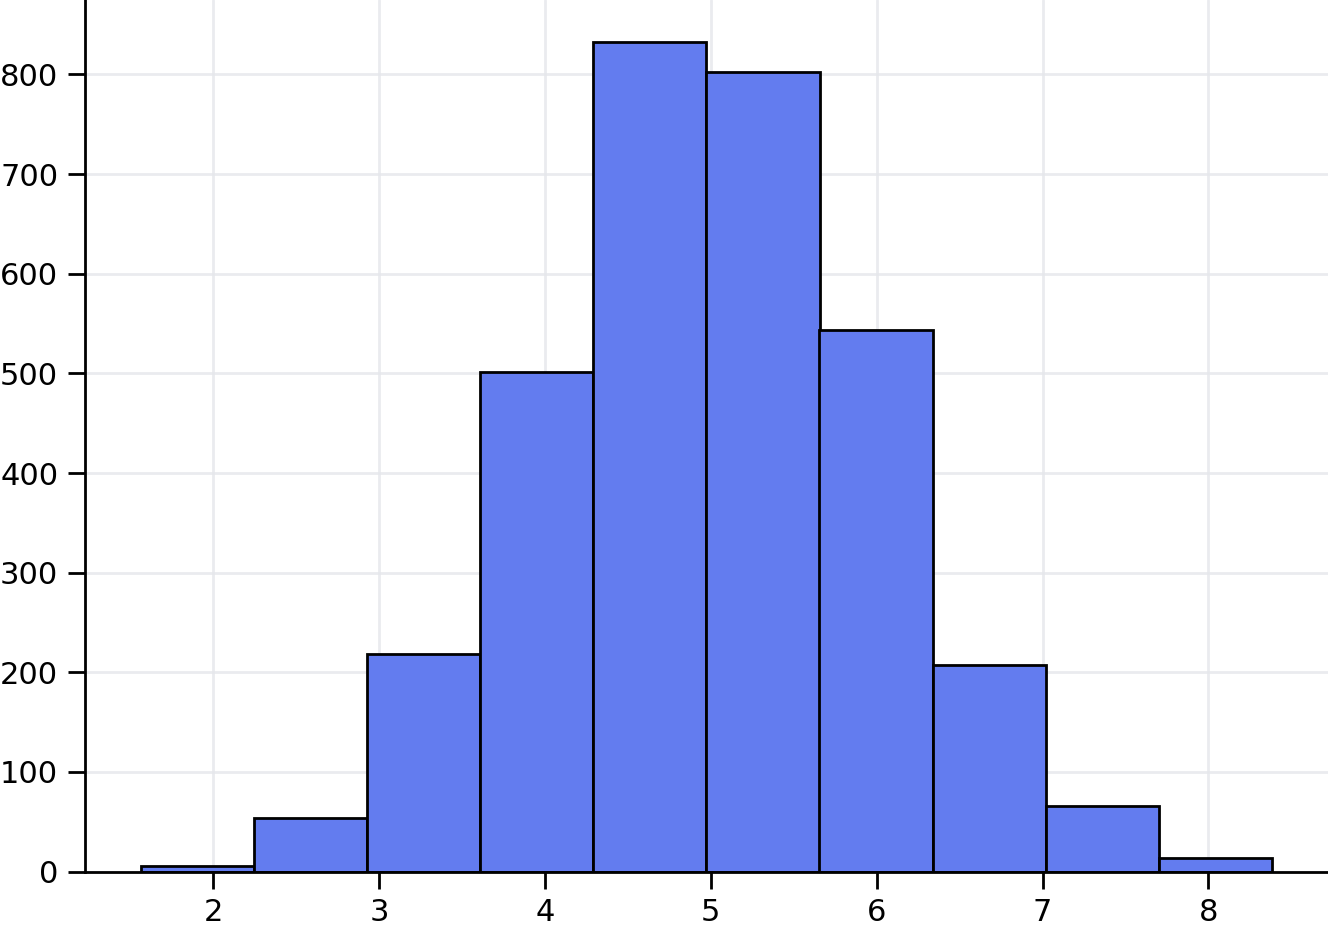
\includegraphics[width=0.78\textwidth]{fig_istogrammami.png}
\caption{Istogramma minimo prodotto da \texttt{istogrammami.py}.}
\label{fig:istogrammami}
\end{figure}

Quando il numero di bin non è specificato, viene utilizzato il valore
predefinito di Matplotlib. Questo script è adatto a un controllo rapido
della distribuzione, ma non documenta ancora le grandezze sugli assi.

\section{Aggiunta delle etichette: \texttt{istogrammami2.py}}

\begin{lstlisting}[language=Python]
import numpy as np
import matplotlib.pyplot as plt

x = np.loadtxt("daterelli.dat")

plt.hist(x)
plt.xlabel("Valore")
plt.ylabel("Conteggi")
plt.show()
\end{lstlisting}

Le istruzioni

\begin{lstlisting}[language=Python]
plt.xlabel("Valore")
plt.ylabel("Conteggi")
\end{lstlisting}

aggiungono rispettivamente il nome dell'asse orizzontale e dell'asse
verticale.

\begin{figure}[htbp]
\centering
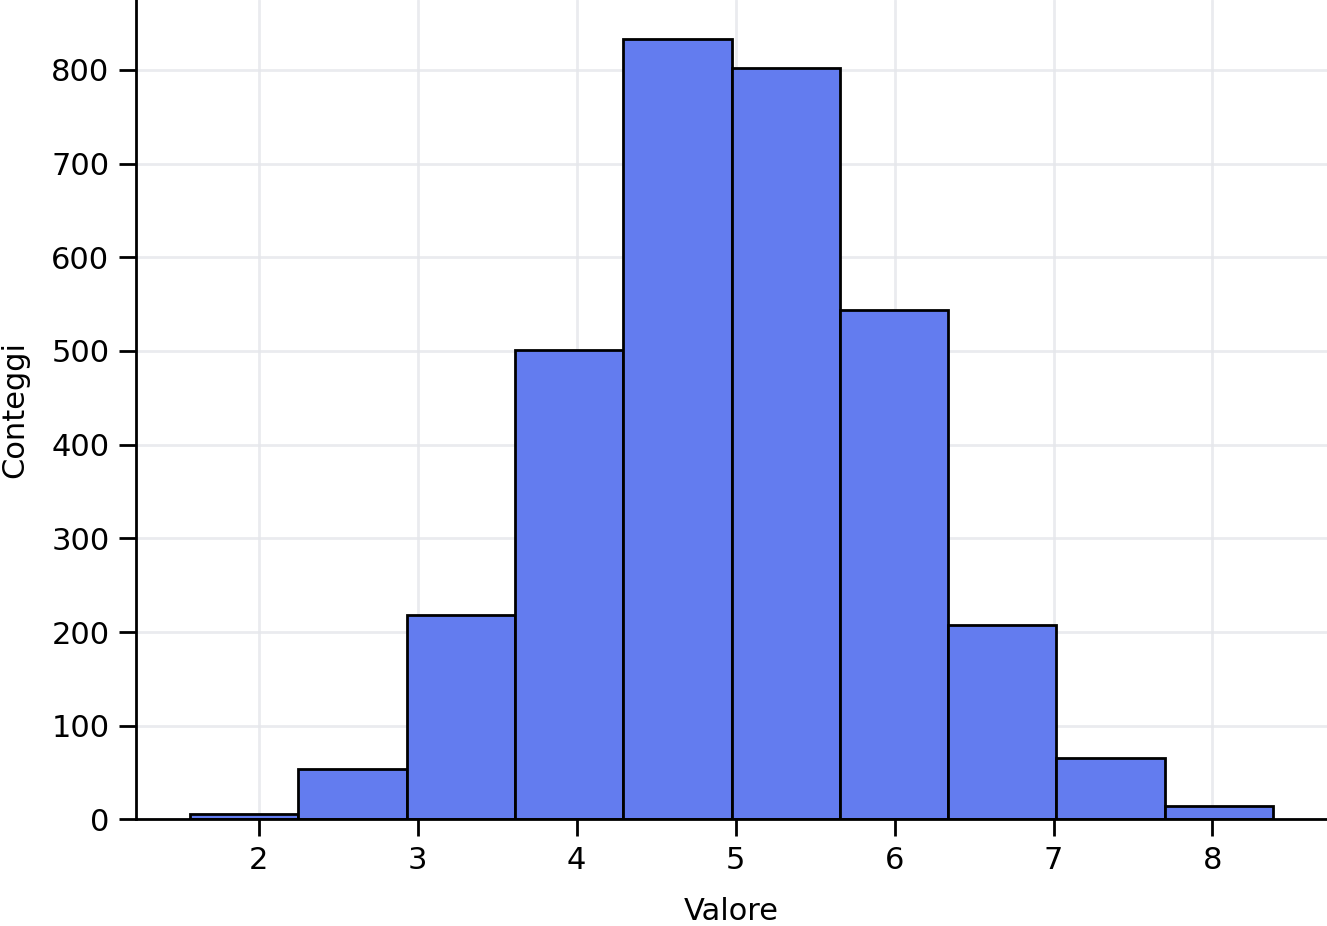
\includegraphics[width=0.78\textwidth]{fig_istogrammami2.png}
\caption{Istogramma con etichette degli assi prodotto da \texttt{istogrammami2.py}.}
\label{fig:istogrammami2}
\end{figure}

La parola \texttt{Conteggi} chiarisce che l'altezza dei bin rappresenta
il numero assoluto di dati. Se si usasse un istogramma normalizzato,
l'etichetta dovrebbe essere modificata, per esempio in
\texttt{Densita di probabilita}.

In una figura scientifica è opportuno specificare anche l'unità di
misura della variabile rappresentata, quando esiste. Per esempio:

\begin{lstlisting}[language=Python]
plt.xlabel("Energia (MeV)")
\end{lstlisting}

\section{Numero di bin e stile: \texttt{istogrammami3.py}}

\begin{lstlisting}[language=Python]
import numpy as np
import matplotlib.pyplot as plt

x = np.loadtxt("daterelli.txt")

plt.hist(
    x,
    bins=20,
    color="skyblue",
    edgecolor="black"
)

plt.xlabel("Valore")
plt.ylabel("Conteggi")
plt.show()
plt.savefig("grafico.pdf")
\end{lstlisting}

\begin{figure}[htbp]
\centering
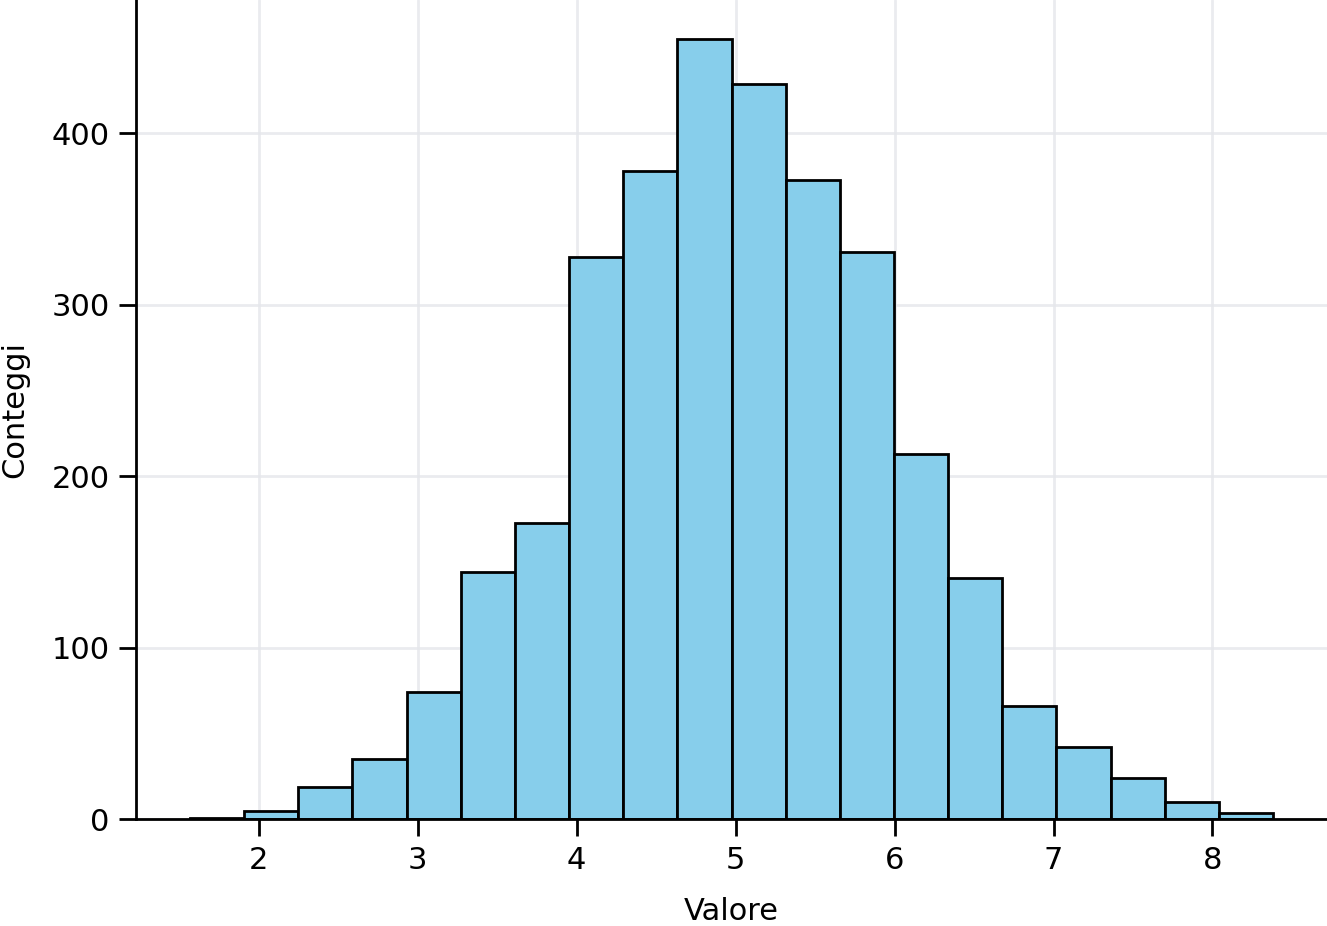
\includegraphics[width=0.78\textwidth]{fig_istogrammami3.png}
\caption{Istogramma a 20 bin con riempimento azzurro e bordi neri.}
\label{fig:istogrammami3}
\end{figure}

\subsection{Scelta del numero di bin}

L'opzione

\begin{lstlisting}[language=Python]
bins=20
\end{lstlisting}

suddivide il campo dei dati in 20 intervalli. La scelta del numero di bin
influenza l'aspetto della distribuzione:

\begin{itemize}
    \item pochi bin producono una rappresentazione molto regolare, ma
          possono nascondere dettagli;
    \item molti bin mostrano più dettagli, ma aumentano le fluttuazioni
          statistiche dei conteggi;
    \item il risultato del successivo fit può dipendere dalla scelta dei
          bin, perché il fit viene effettuato sui conteggi raggruppati.
\end{itemize}

\subsection{Colore e bordi}

L'opzione

\begin{lstlisting}[language=Python]
color="skyblue"
\end{lstlisting}

imposta il colore interno delle barre. L'opzione

\begin{lstlisting}[language=Python]
edgecolor="black"
\end{lstlisting}

rende neri i bordi, migliorando la separazione visiva tra bin
consecutivi.

\subsection{Salvataggio della figura}

Lo script usa

\begin{lstlisting}[language=Python]
plt.savefig("grafico.pdf")
\end{lstlisting}

per salvare la figura in PDF. È preferibile salvare la figura prima di
\texttt{plt.show()}:

\begin{lstlisting}[language=Python]
plt.savefig("grafico.pdf")
plt.show()
\end{lstlisting}

Alcuni backend possono infatti modificare o chiudere la figura corrente
dopo la visualizzazione.

\section{Che cos'è un fit}

Un \emph{fit} determina i parametri di un modello matematico in modo che
il modello descriva nel modo migliore possibile i dati osservati.

Nel nostro caso, i dati grezzi vengono prima raggruppati in un
istogramma. Il fit non viene applicato direttamente alle barre come
oggetti grafici, ma alle coppie numeriche

\[
(x_i,N_i),
\]

dove:

\begin{itemize}
    \item $x_i$ è il centro del bin $i$;
    \item $N_i$ è il conteggio del bin $i$.
\end{itemize}

Si sceglie quindi una funzione $f(x;\boldsymbol{p})$, dipendente da un
insieme di parametri $\boldsymbol{p}$, e si cercano i valori dei
parametri che rendono piccole le differenze tra i conteggi osservati e i
valori previsti dal modello.

Queste differenze sono dette \emph{residui}:

\[
r_i=N_i-f(x_i;\boldsymbol{p}).
\]

Se ogni conteggio possiede un'incertezza $\sigma_i$, si può minimizzare
il chi-quadro

\[
\chi^2(\boldsymbol{p})=
\sum_i
\left[
\frac{N_i-f(x_i;\boldsymbol{p})}{\sigma_i}
\right]^2.
\]

Per conteggi sufficientemente grandi si usa spesso l'approssimazione
poissoniana

\[
\sigma_i\simeq\sqrt{N_i}.
\]

I bin con $N_i=0$ hanno, con questa formula, errore nullo. Lo script
considerato sostituisce tali errori con 1 per evitare una divisione per
zero. Un'altra possibilità consiste nell'escludere i bin vuoti mediante
una maschera booleana.

\section{Il modello gaussiano}

Il modello utilizzato è

\[
g(x;A,\mu,\sigma)=
A\exp\left[-\frac{(x-\mu)^2}{2\sigma^2}\right].
\]

I parametri hanno il seguente significato:

\begin{itemize}
    \item $A$ è l'altezza della gaussiana nel punto di massimo;
    \item $\mu$ è la posizione del centro e del massimo;
    \item $\sigma$ controlla la larghezza della distribuzione.
\end{itemize}

La funzione usata nello script non è una densità normalizzata a area
unitaria. Essa descrive direttamente l'altezza dei conteggi. Perciò $A$
è l'altezza del picco e non il numero totale di eventi.

\section{Istogramma e fit gaussiano: \texttt{istogrammafit.py}}

\begin{lstlisting}[language=Python]
import numpy as np
import matplotlib.pyplot as plt
from scipy.optimize import curve_fit

# funzione gaussiana
def gaussiana(x, A, mu, sigma):
    return A * np.exp(-(x - mu)**2 / (2 * sigma**2))

# lettura dati
x = np.loadtxt("daterelli.txt")

# istogramma
conteggi, bin_edges, _ = plt.hist(
    x,
    bins=20,
    color="skyblue",
    edgecolor="black",
    label="Dati"
)

# centri dei bin
bin_centri = (bin_edges[:-1] + bin_edges[1:]) / 2

# errori poissoniani
errori = np.sqrt(conteggi)
errori[errori == 0] = 1

# parametri iniziali
A0 = np.max(conteggi)
mu0 = np.mean(x)
sigma0 = np.std(x)

# fit gaussiano
popt, pcov = curve_fit(
    gaussiana,
    bin_centri,
    conteggi,
    p0=[A0, mu0, sigma0],
    sigma=errori,
    absolute_sigma=True
)

# errori sui parametri
perr = np.sqrt(np.diag(pcov))

# curva liscia
xfit = np.linspace(
    bin_edges[0],
    bin_edges[-1],
    500
)

yfit = gaussiana(xfit, *popt)

# disegno del fit
plt.plot(
    xfit,
    yfit,
    "r-",
    lw=2,
    label="Fit gaussiano"
)

plt.xlabel("Valore")
plt.ylabel("Conteggi")
plt.legend()

# stampa risultati
print("\nFit gaussiano")
print(f"A     = {popt[0]:.5g} +/- {perr[0]:.2g}")
print(f"mu    = {popt[1]:.5g} +/- {perr[1]:.2g}")
print(f"sigma = {popt[2]:.5g} +/- {perr[2]:.2g}")

plt.savefig("grafico.pdf")
plt.savefig("grafico.png", dpi=300)
plt.show()
\end{lstlisting}

\begin{figure}[htbp]
\centering
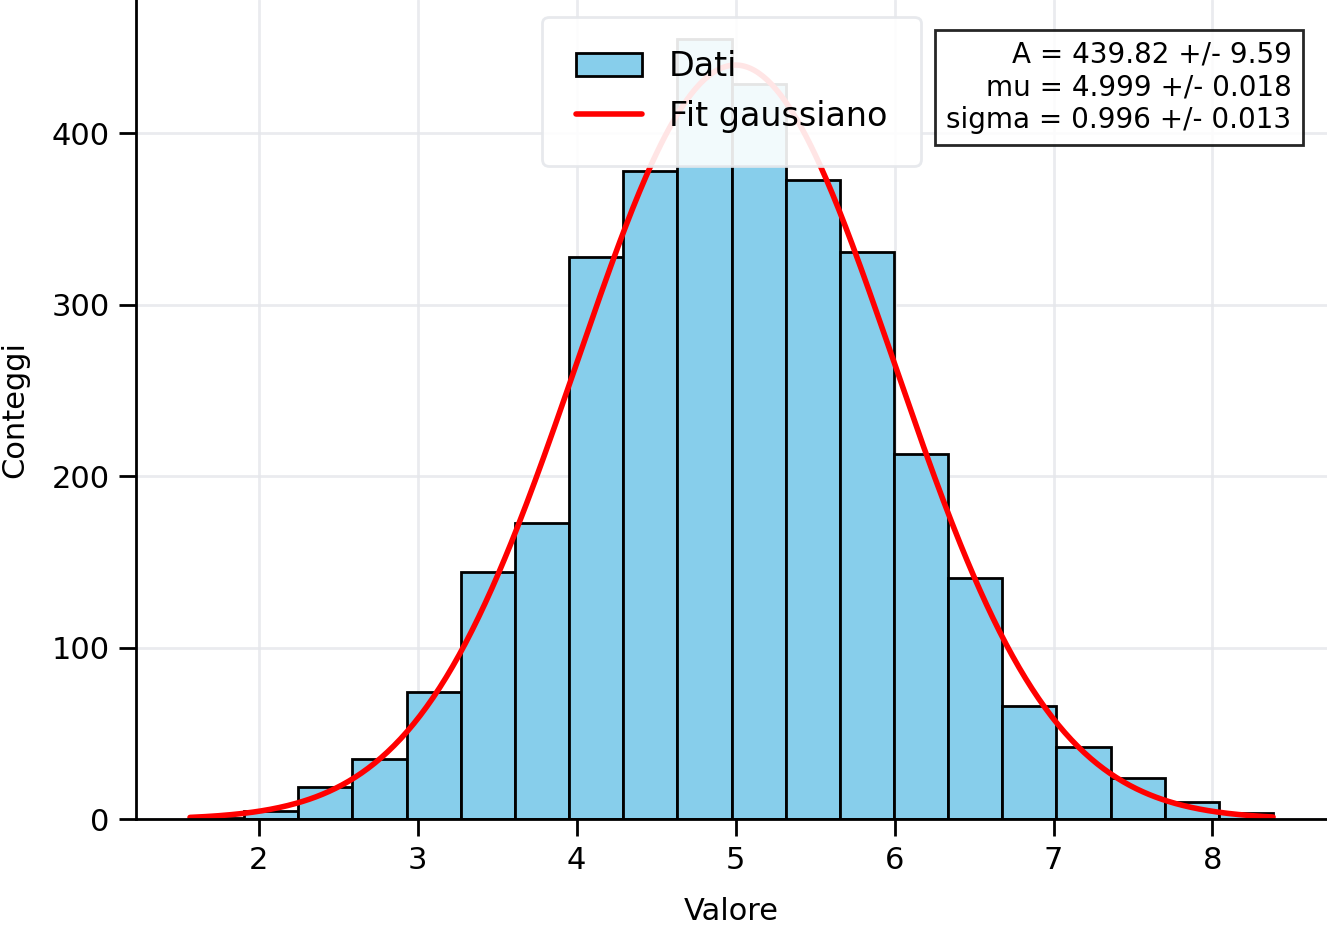
\includegraphics[width=0.82\textwidth]{fig_istogramma_fit.png}
\caption{Istogramma dei dati con sovrapposto il fit gaussiano.}
\label{fig:istogramma-fit}
\end{figure}

\subsection{Importazione di \texttt{curve\_fit}}

L'istruzione

\begin{lstlisting}[language=Python]
from scipy.optimize import curve_fit
\end{lstlisting}

importa la funzione di SciPy che determina i parametri ottimali del
modello.

\subsection{Definizione della funzione}

La funzione

\begin{lstlisting}[language=Python]
def gaussiana(x, A, mu, sigma):
    return A * np.exp(-(x - mu)**2 / (2 * sigma**2))
\end{lstlisting}

ha come primo argomento la variabile indipendente e, successivamente, i
parametri da determinare. Questa è la forma richiesta da
\texttt{curve\_fit}.

L'operazione \texttt{(x-mu)**2} è vettoriale: se \texttt{x} è un array,
NumPy calcola contemporaneamente il valore della gaussiana in tutti i
punti.

\subsection{Valori restituiti da \texttt{plt.hist}}

A differenza degli script precedenti, il risultato di \texttt{plt.hist}
non viene ignorato:

\begin{lstlisting}[language=Python]
conteggi, bin_edges, _ = plt.hist(...)
\end{lstlisting}

La funzione restituisce tre oggetti:

\begin{itemize}
    \item \texttt{conteggi}: numero di elementi in ogni bin;
    \item \texttt{bin\_edges}: bordi dei bin;
    \item il terzo oggetto contiene le barre grafiche; viene assegnato a
          \texttt{\_} perché non viene utilizzato.
\end{itemize}

Questa riga mostra chiaramente il doppio ruolo di \texttt{plt.hist}:
calcola l'istogramma e contemporaneamente lo disegna. Il fit successivo
usa \texttt{conteggi} e \texttt{bin\_edges}, non le barre grafiche.

\subsection{Calcolo dei centri dei bin}

Se i bordi sono

\[
b_0,b_1,\ldots,b_m,
\]

il centro del bin $i$ è

\[
x_i=\frac{b_i+b_{i+1}}{2}.
\]

In NumPy:

\begin{lstlisting}[language=Python]
bin_centri = (bin_edges[:-1] + bin_edges[1:]) / 2
\end{lstlisting}

L'espressione \texttt{bin\_edges[:-1]} contiene tutti i bordi tranne
l'ultimo; \texttt{bin\_edges[1:]} contiene tutti i bordi tranne il primo.
La somma elemento per elemento accoppia quindi il bordo sinistro e il
bordo destro di ciascun bin.

\subsection{Errori poissoniani e maschera}

Gli errori sono stimati mediante

\begin{lstlisting}[language=Python]
errori = np.sqrt(conteggi)
\end{lstlisting}

La riga

\begin{lstlisting}[language=Python]
errori[errori == 0] = 1
\end{lstlisting}

usa una maschera booleana. La condizione \texttt{errori == 0} seleziona
gli elementi nulli; l'assegnazione li sostituisce con 1. Ciò impedisce
che nel chi-quadro compaia una divisione per zero.

Una variante che esclude i bin vuoti è:

\begin{lstlisting}[language=Python]
maschera = conteggi > 0

centri_fit = bin_centri[maschera]
conteggi_fit = conteggi[maschera]
errori_fit = np.sqrt(conteggi[maschera])
\end{lstlisting}

In tal caso, i tre array filtrati devono essere passati a
\texttt{curve\_fit}.

\subsection{Stime iniziali}

La procedura di minimizzazione ha bisogno di valori iniziali:

\begin{lstlisting}[language=Python]
A0 = np.max(conteggi)
mu0 = np.mean(x)
sigma0 = np.std(x)
\end{lstlisting}

Le scelte sono naturali:

\begin{itemize}
    \item il massimo conteggio approssima l'altezza del picco;
    \item la media campionaria approssima il centro;
    \item la deviazione standard campionaria approssima la larghezza.
\end{itemize}

Questi valori vengono raccolti, nello stesso ordine degli argomenti della
funzione, in

\begin{lstlisting}[language=Python]
p0=[A0, mu0, sigma0]
\end{lstlisting}

\subsection{Esecuzione del fit}

La chiamata principale è

\begin{lstlisting}[language=Python]
popt, pcov = curve_fit(
    gaussiana,
    bin_centri,
    conteggi,
    p0=[A0, mu0, sigma0],
    sigma=errori,
    absolute_sigma=True
)
\end{lstlisting}

Gli argomenti indicano:

\begin{itemize}
    \item il modello da adattare;
    \item le ascisse dei punti, cioè i centri dei bin;
    \item le ordinate, cioè i conteggi;
    \item le stime iniziali dei parametri;
    \item le incertezze dei conteggi;
    \item l'interpretazione assoluta delle incertezze fornite.
\end{itemize}

L'array \texttt{popt} contiene i parametri ottimali:

\[
\texttt{popt}=[A,\mu,\sigma].
\]

La matrice \texttt{pcov} è la matrice di covarianza dei parametri.

\subsection{Matrice di covarianza e incertezze}

Per tre parametri, la matrice ha la forma

\[
\mathbf{C}=
\begin{pmatrix}
\operatorname{Var}(A) & \operatorname{Cov}(A,\mu) &
\operatorname{Cov}(A,\sigma)\\
\operatorname{Cov}(\mu,A) & \operatorname{Var}(\mu) &
\operatorname{Cov}(\mu,\sigma)\\
\operatorname{Cov}(\sigma,A) & \operatorname{Cov}(\sigma,\mu) &
\operatorname{Var}(\sigma)
\end{pmatrix}.
\]

Gli elementi diagonali sono le varianze dei parametri. Le incertezze
standard sono quindi

\[
\delta p_i=\sqrt{C_{ii}}.
\]

Nel codice:

\begin{lstlisting}[language=Python]
perr = np.sqrt(np.diag(pcov))
\end{lstlisting}

Gli elementi fuori diagonale descrivono invece le correlazioni tra le
stime dei parametri.

\subsection{Disegno di una curva regolare}

Il fit è stato eseguito nei centri dei bin, ma per disegnare una curva
regolare si genera una griglia più fitta:

\begin{lstlisting}[language=Python]
xfit = np.linspace(
    bin_edges[0],
    bin_edges[-1],
    500
)
\end{lstlisting}

La funzione gaussiana viene valutata nei 500 punti:

\begin{lstlisting}[language=Python]
yfit = gaussiana(xfit, *popt)
\end{lstlisting}

L'asterisco in \texttt{*popt} spacchetta l'array. L'istruzione equivale a

\begin{lstlisting}[language=Python]
yfit = gaussiana(
    xfit,
    popt[0],
    popt[1],
    popt[2]
)
\end{lstlisting}

La curva viene infine sovrapposta in rosso all'istogramma.

\subsection{Stampa dei risultati}

Le f-string

\begin{lstlisting}[language=Python]
print(f"A     = {popt[0]:.5g} +/- {perr[0]:.2g}")
print(f"mu    = {popt[1]:.5g} +/- {perr[1]:.2g}")
print(f"sigma = {popt[2]:.5g} +/- {perr[2]:.2g}")
\end{lstlisting}

stampano cinque cifre significative per i parametri e due per le
incertezze. Nello script Python originale il simbolo \texttt{+/-} può
essere sostituito dal carattere Unicode \texttt{±}, se il terminale e il
file sorgente usano una codifica compatibile.

\section{Osservazioni statistiche}

Il fit presentato è un fit ai conteggi raggruppati. La scelta dei bin
influenza sia le ascisse del fit sia i conteggi. Due istogrammi costruiti
con numeri di bin differenti possono quindi produrre parametri
leggermente differenti.

L'approssimazione $\sqrt{N_i}$ è più affidabile quando i conteggi non
sono troppo piccoli. Per conteggi bassi o numerosi bin vuoti, una
trattazione poissoniana basata sulla verosimiglianza è in genere più
adeguata del chi-quadro gaussiano. Nel contesto didattico corrente,
questa procedura permette comunque di collegare in modo trasparente:

\begin{center}
\texttt{dati grezzi}
$\longrightarrow$
\texttt{istogramma}
$\longrightarrow$
\texttt{conteggi e centri}
$\longrightarrow$
\texttt{fit gaussiano}.
\end{center}

\section{Riepilogo}

Il percorso seguito mostra progressivamente che:

\begin{enumerate}
    \item un istogramma è innanzitutto un algoritmo di conteggio;
    \item \texttt{plt.hist} calcola i conteggi e disegna le barre;
    \item \texttt{bins} controlla la suddivisione dell'intervallo;
    \item i valori restituiti da \texttt{plt.hist} possono essere usati
          in calcoli successivi;
    \item il fit non usa direttamente gli oggetti grafici, ma i centri e
          i conteggi dei bin;
    \item \texttt{curve\_fit} restituisce i parametri ottimali e la loro
          matrice di covarianza;
    \item la diagonale della matrice di covarianza permette di ricavare
          le incertezze sui parametri.
\end{enumerate}
